\section{Analysis tasks}
TODO: write something here
\subsection{Stream signatures}
\label{sec:stream-signature}

To analyze the core characteristics of a stream, we introduce the concept of a stream
\emph{signature}. A signature is a $B \times L$ matrix, with $B$ being the number of bit planes, and
$S$ being the number of subbands produced by the wavelet transform. A chunk on subband $s$ and bit
plane $b$ can be associated with the $b, l$ cell of the matrix. Every chunk in the stream can be
associated with one (and only one) of the cells. Each matrix cell $(b,l)$ contains a value in the
range of $[0,B\times L)$, indicating the position in which chunks of that cell appear in the stream,
relative to chunks of all other cells, on average. It is our hypothesis that streams optimized for
different analysis tasks produce qualitatively distinctive signatures, and therefore, a set of
signatures can be pre-computed once and later picked to use depending on the analysis at hand.

To compute a stream signature, we partition the whole domain into several regions, compute one
chunks in each per-region signature are spatially related. The reason for this partitioning is that
it is only meaningful to study the relative ordering of cells if the chunks associated with those
cells all come from same region of the original domain. Ideally the global signature for a stream
should contain all the per-region signatures, but due to space constraint, as well as for ease of
visualization, we condense all the local signatures by averaging them on a per-cell basis, and only
study the average signature. (TODO: add the algorithm).

\subsection{Function reconstruction}
\label{sec:rmse-optimized}

The most fundamental task is that of reconstructing the function itself (i.e., $Q$ is the identity
map), using a common error metric such as the root-mean-square error (RMSE). For each data set, we
use the aforementioned $O(n)$ greedy algorithm to construct an \emph{rmse-optimized} stream. In
Section \ref{sec:motivation} we have seen that the \emph{by wavelet norm} performs the best among
the data-agnostic streams with regards to RMSE. To see how the \emph{rmse-optimized} stream, which
is data-dependent, compares to the data-agnostic streams, we plot all four streams together in
Figure \ref{fig:rmse-optimized}. It can be seen that the difference between \emph{by wavelet norm}
and \emph{rmse-optimized} is negligible in most cases. This result is expected, because \emph{by
wavelet norm} and \emph{rmse-optimized} both order the chunks according to their contribution to in
the $L_2$ sense, with \emph{rmse-optimized} also taking into account the actual values of the bits.
This difference has little effect in this case, because, as leading zero bits are removed, the rest
of the bits (of the wavelet coefficients) are known to be distributed approximately uniformly among
$0$ and $1$ for wavelet coefficients [CITE]. 

Among the static streams, \emph{by level} performs poorly compared to \emph{by bit plane} and
\emph{by wavelet norm}. This is because, in the $L_2$ norm, low-ordered bits or coarse-level
coefficients contribute little compared to high-ordered bits of fine-level coefficients. This
difference in contribution is magnified when the data contains fine-scale features, as is the case
for the \emph{plasma} data set. In Figure \ref{fig:rmse-rendering}, we render this field at 0.74
bits per sample for all three streams, and compare these rendering with that of the groundtruth
data. \emph{by level} results in heavy artifacts that are not seen by \emph{by bit plane} and
\emph{by wavelet norm}. \emph{by wavelet norm} performs slightly better than \emph{by bit plane}
here and in all other cases. These results suggest that in practice, \emph{by wavelet norm} is a
near-optimal way to stream data that minimizes root-mean-square errors, regardless of the data.

\begin{figure}[h]
  \centering
	\subcaptionbox{Boiler}
  {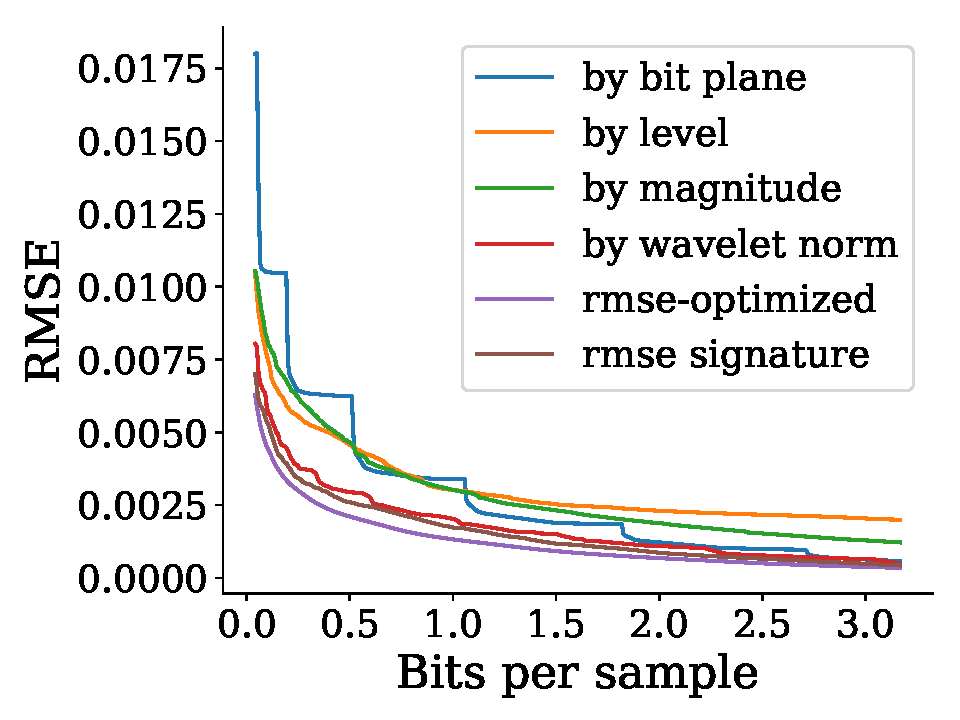
\includegraphics[width=0.48\linewidth]{img/rmse/rmse-optimized-boiler.pdf}}
	\subcaptionbox{Diffusivity}
 	{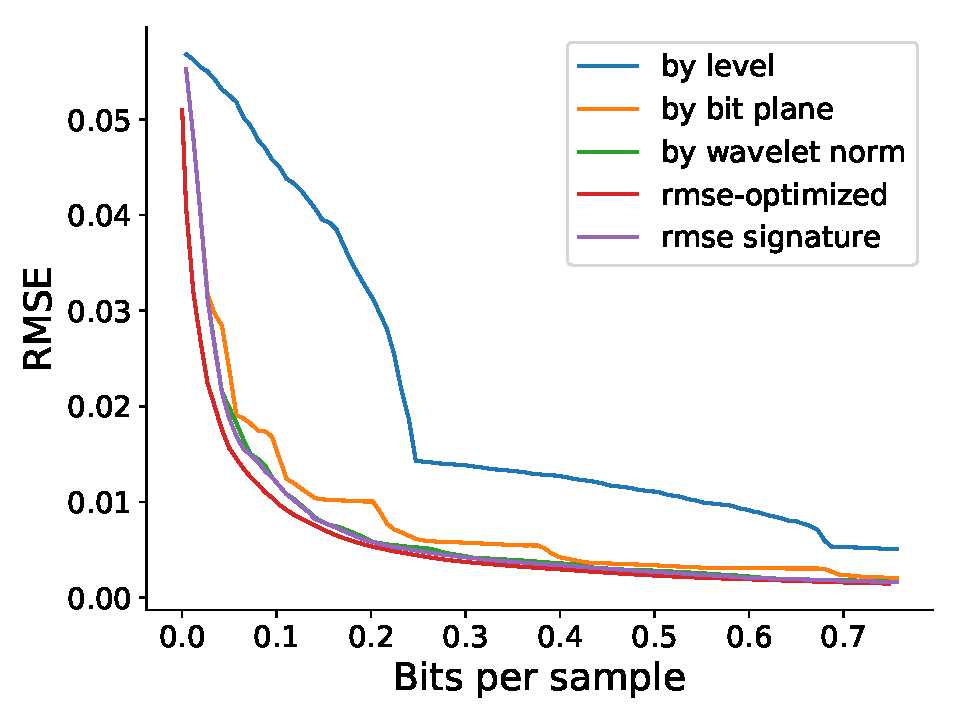
\includegraphics[width=0.48\linewidth]{img/rmse/rmse-optimized-diffusivity.pdf}}
	\subcaptionbox{Euler}
 	{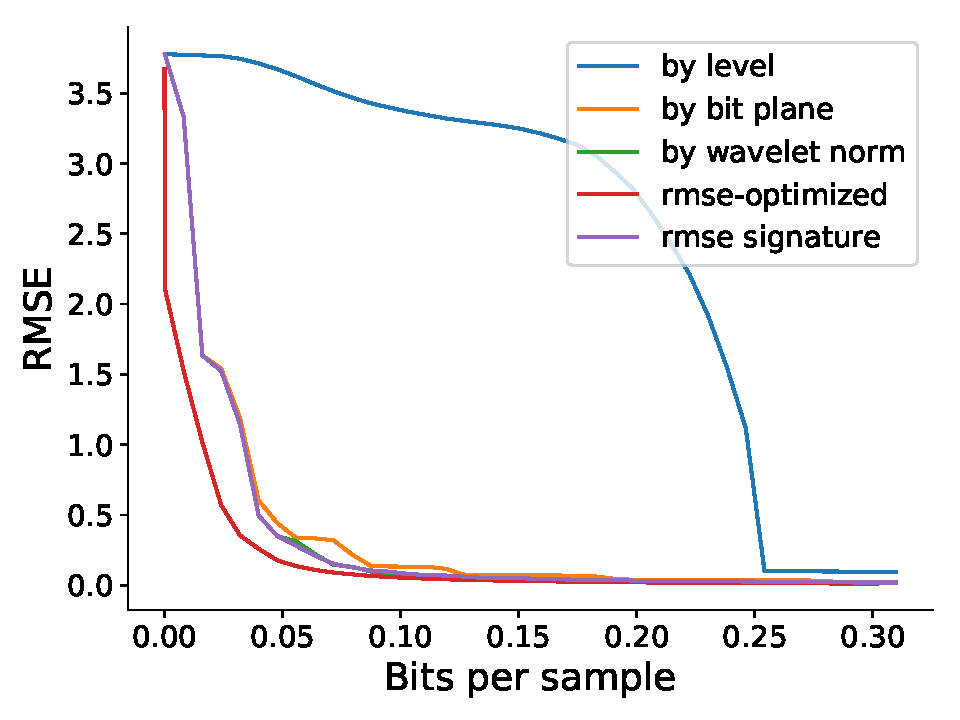
\includegraphics[width=0.48\linewidth]{img/rmse/rmse-optimized-euler.pdf}}
	\subcaptionbox{Turbulence}
 	{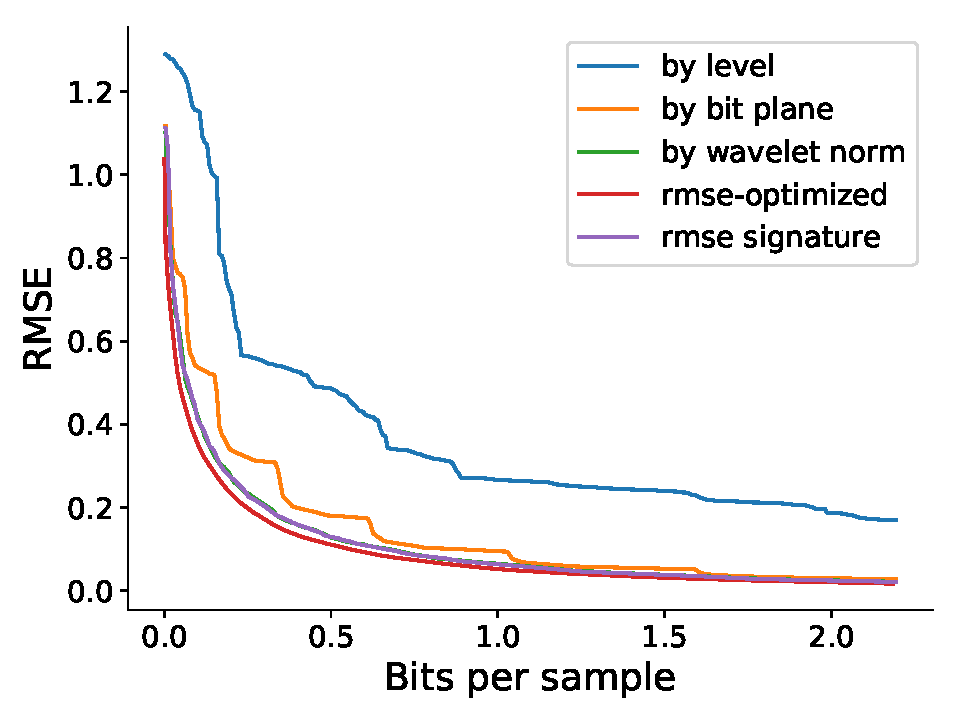
\includegraphics[width=0.48\linewidth]{img/rmse/rmse-optimized-turbulence.pdf}}
	\subcaptionbox{Plasma}
 	{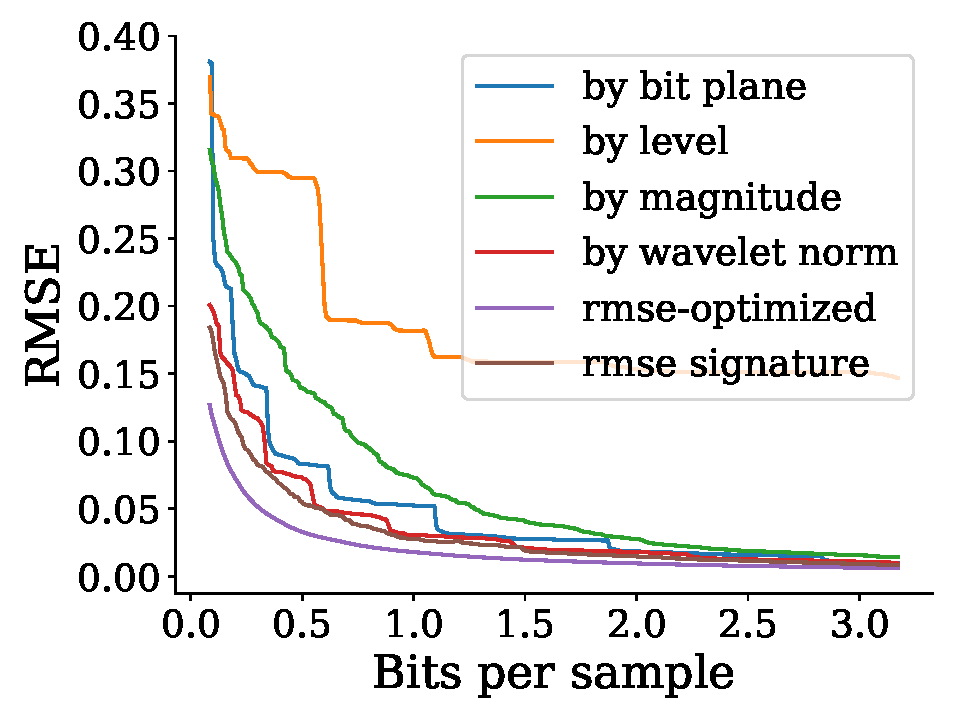
\includegraphics[width=0.48\linewidth]{img/rmse/rmse-optimized-plasma.pdf}}
	\subcaptionbox{Velocity-z}
 	{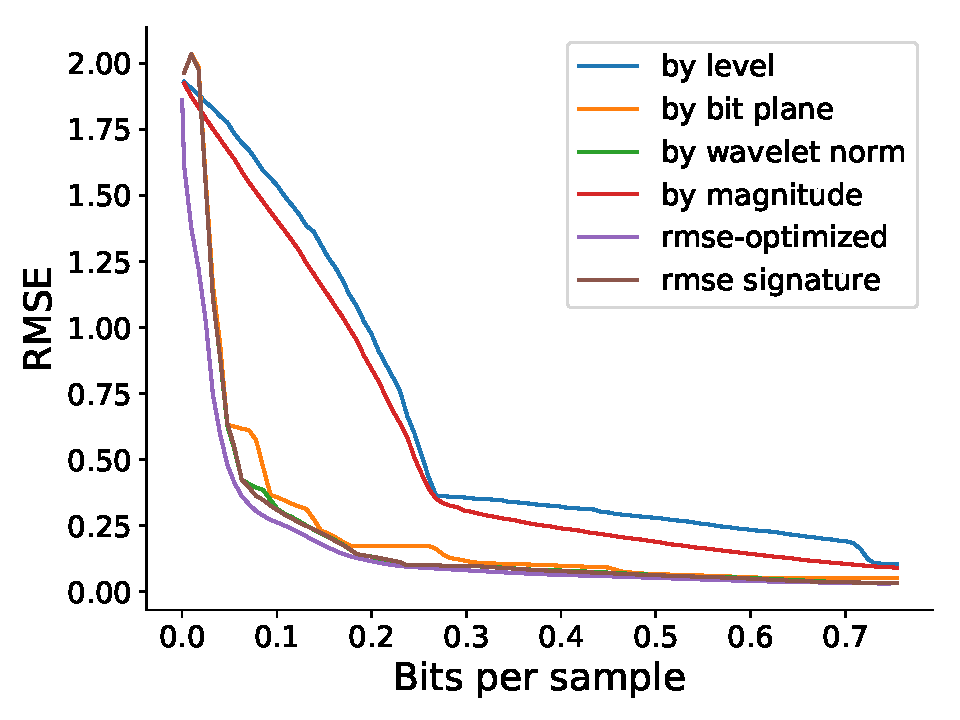
\includegraphics[width=0.48\linewidth]{img/rmse/rmse-optimized-velocityz.pdf}}
 	\caption{Root-mean-square error of reconstructed functions for the three data-agnostic streams
 	defined in Section \ref{sec:motivation}, and the \emph{rmse-optimized} stream. Lower is better.
 	The streams are truncated to highlight the differences, without omitting important information.
 	\emph{rmse-optimized} performs best, followed closely by \emph{by wavelet norm} and \emph{by bit
 	plane}.}
 	\label{fig:rmse-optimized}
\end{figure}

\begin{figure}[h]
	\centering
	{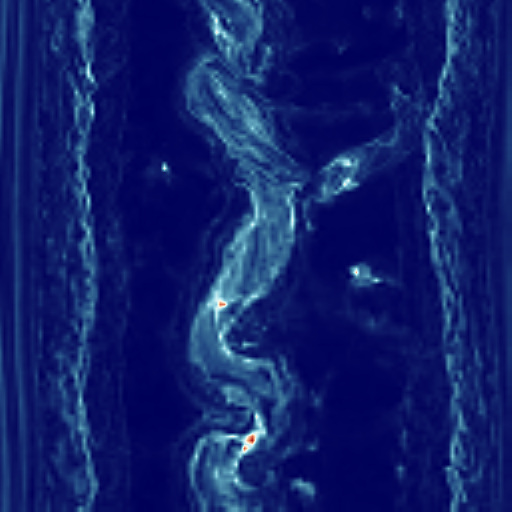
\includegraphics[width=0.24\linewidth]{img/rmse/plasma_curr_func2.png}}
	{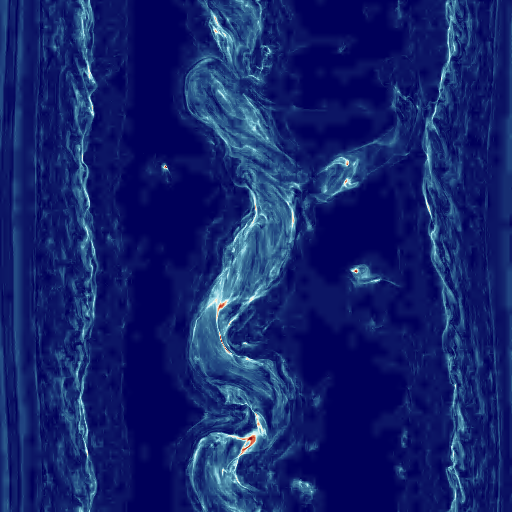
\includegraphics[width=0.24\linewidth]{img/rmse/plasma_curr_func1.png}}
	{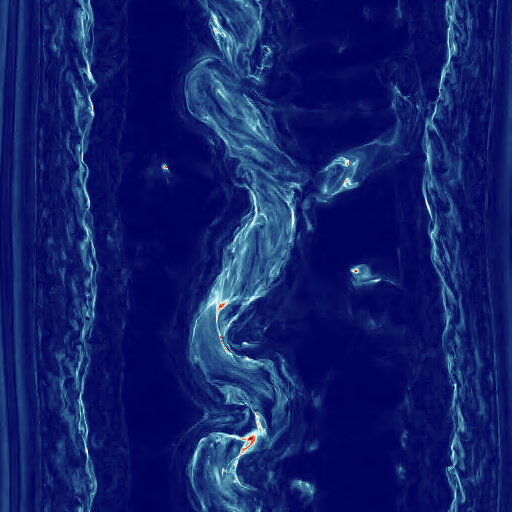
\includegraphics[width=0.24\linewidth]{img/rmse/plasma_curr_func0.png}}
	{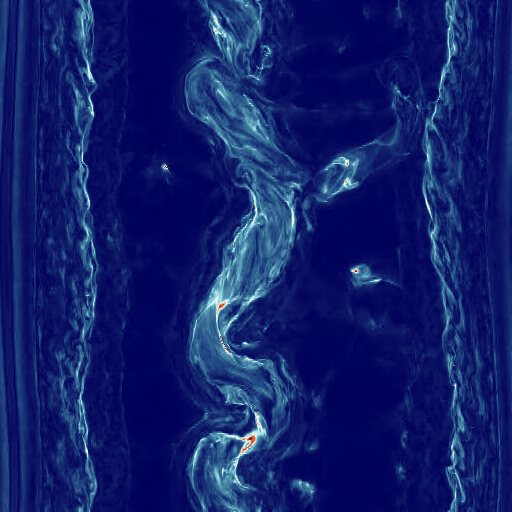
\includegraphics[width=0.24\linewidth]{img/rmse/signature_curr_func0.png}}
	{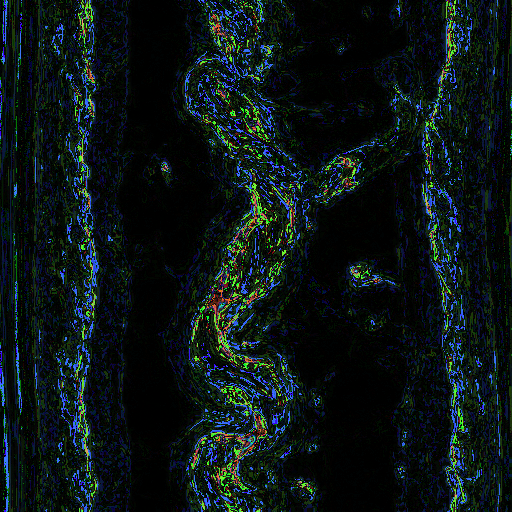
\includegraphics[width=0.24\linewidth]{img/rmse/plasma_curr_func2_diff.png}}
	{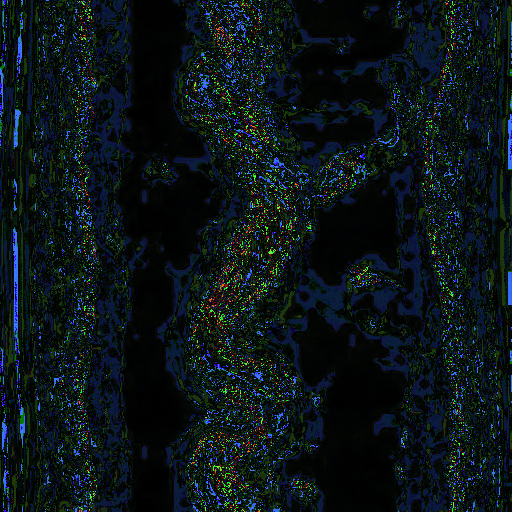
\includegraphics[width=0.24\linewidth]{img/rmse/plasma_curr_func1_diff.png}}
	{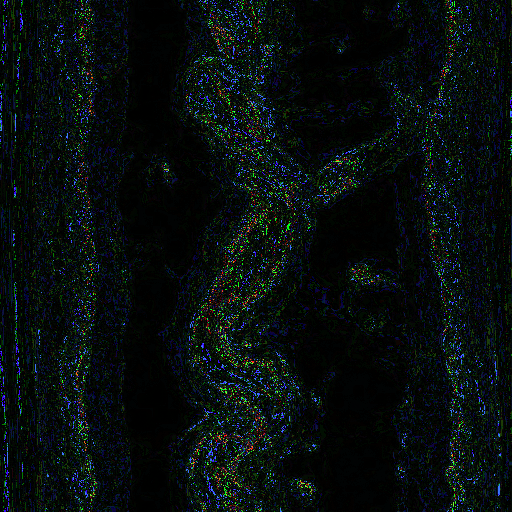
\includegraphics[width=0.24\linewidth]{img/rmse/plasma_curr_func0_diff.png}}
	{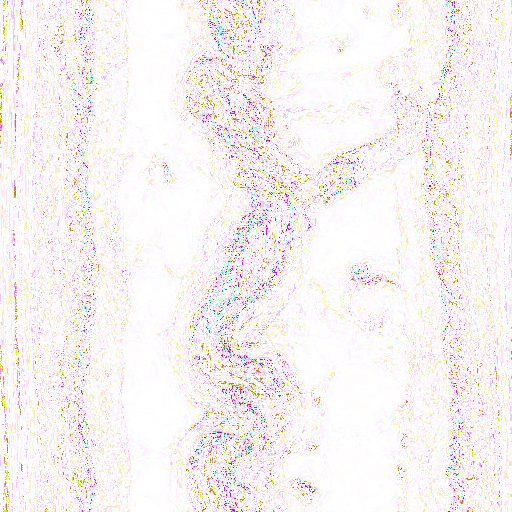
\includegraphics[width=0.24\linewidth]{img/rmse/signature_curr_func0_diff.png}}
	
	\caption{Top row:	renderings of the \emph{plasma} function at 0.74 bps. From left to right:
	\emph{by level}, \emph{by bit plane}, \emph{by wavelet norm}, and ground-truth. Bottom row:
	difference (XOR) of the reconstructed images (in respective order) from the groundtruth image,
	brighter pixels mean higher errors. The \emph{by wavelet norm} provides the most accurate
	function, followed closely by
	\emph{by bit plane}.}
 	\label{fig:rmse-rendering}
\end{figure}

\begin{figure}[h]
	\centering
	{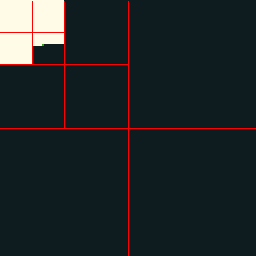
\includegraphics[width=0.24\linewidth]{img/rmse/rmse-precision-dist-by-level.png}}
	{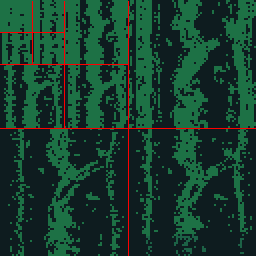
\includegraphics[width=0.24\linewidth]{img/rmse/rmse-precision-by-bit-plane.png}}
	{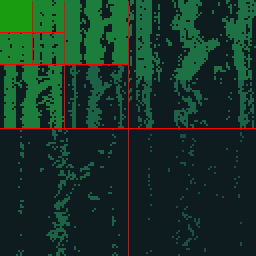
\includegraphics[width=0.24\linewidth]{img/rmse/rmse-precision-dist-by-wavelet-norm.png}}
	{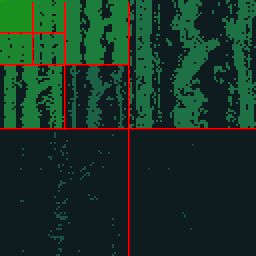
\includegraphics[width=0.24\linewidth]{img/rmse/rmse-precision-signature.png}}
	
	\caption{Precision distribution, plasma, 0.74 bps.}
 	\label{fig:rmse-rendering}
\end{figure}
